\QCMautoevaluation{Pour chaque question, plusieurs réponses sont proposées. Déterminer celles qui sont correctes.}

\begin{QCM}

\begin{GroupeQCM}


\begin{exercice}
Parmi les couples d'angles suivants, quels sont ceux qui sont complémentaires ?
\begin{ChoixQCM}{2}
\item $\widehat{FEG}=8$° et $\widehat{HIK}=82$°
\item $\widehat{FEG}=90$° et $\widehat{HIK}=90$°
\item $\widehat{ABC}=73$° et $\widehat{STU}=107$°
\item $\widehat{FEG}=89,9$° et $\widehat{HIK}=0,1$°
\end{ChoixQCM}
\begin{corrige}
\reponseQCM{a}
\end{corrige}
\end{exercice}
\end{GroupeQCM}



\begin{EnonceCommunQCM}
Les questions \RefQCM{Aqcm1} et \RefQCM{Aqcm2} se rapportent à la figure ci-dessous.
\begin{center}
    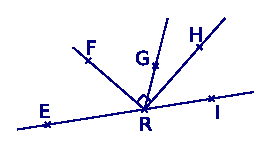
\includegraphics[width=.25\linewidth]{qcm1}
    
    $E$, $R$ et $I$ sont alignés.
\end{center}
\end{EnonceCommunQCM}

\begin{GroupeQCM}


\begin{exercice}\label{Aqcm1}
Les angles...
\begin{ChoixQCM}{2}
\item $\widehat{ERH}$ et $\widehat{HRI}$ sont supplémentaires
\item $\widehat{FRG}$ et $\widehat{HRI}$ sont adjacents
\item $\widehat{ERG}$ et $\widehat{FRI}$ sont supplémentaires
\item $\widehat{FRG}$ et $\widehat{GRH}$ sont adjacents
\end{ChoixQCM}
\begin{corrige}
\reponseQCM{a}
\end{corrige}
\end{exercice}





\begin{exercice}\label{Aqcm2}
L'angle...
\begin{ChoixQCM}{2}
\item $\widehat{FRG}$ est le complémentaire de $\widehat{GRH}$
\item $\widehat{FRE}$ est le complémentaire de $\widehat{HRI}$
\item $\widehat{ERF}$ est le complémentaire de $\widehat{FRI}$
\item $\widehat{GRH}$ est le complémentaire de $\widehat{HRI}$
\end{ChoixQCM}
\begin{corrige}
\reponseQCM{a}
\end{corrige}
\end{exercice}
\end{GroupeQCM}
\end{QCM}

\begin{QCM}

\begin{EnonceCommunQCM}
Les questions \RefQCM{Aqcm3}, \RefQCM{Aqcm4} et \RefQCM{Aqcm5} se rapportent à la figure ci-dessous.
\begin{center}
    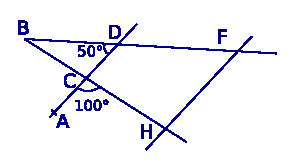
\includegraphics[width=.25\linewidth]{qcm2}
    
    $(AD)$ et $(FH)$ sont parallèles.
\end{center}
\end{EnonceCommunQCM}

\begin{GroupeQCM}

\begin{exercice}\label{Aqcm3}

\begin{ChoixQCM}{2}
\item $\widehat{ACH}$ et $\widehat{BCD}$ sont opposés par le sommet
\item $\widehat{CDF}$ et $\widehat{BCD}$ sont opposés par le sommet
\item $\widehat{ACH}$ et $\widehat{BCD}$ sont adjacents
\item $\widehat{BCD}$ et $\widehat{CHF}$ sont correspondants
\end{ChoixQCM}
\begin{corrige}
\reponseQCM{a}
\end{corrige}
\end{exercice}




\begin{exercice}\label{Aqcm4}

\begin{ChoixQCM}{4}
\item $\widehat{BCD}=100$°
\item $\widehat{BHF}=100$°
\item $\widehat{BCA}=100$°
\item $\widehat{DCH}=100$°
\end{ChoixQCM}
\begin{corrige}
\reponseQCM{a}
\end{corrige}
\end{exercice}




\begin{exercice}\label{Aqcm5}

\begin{ChoixQCM}{4}
\item $\widehat{CDF}=40$°
\item $\widehat{BFH}=50$°
\item $\widehat{DCH}=80$°
\item $\widehat{CDF}=100$°
\end{ChoixQCM}
\begin{corrige}
\reponseQCM{a}
\end{corrige}
\end{exercice}

\end{GroupeQCM}
\end{QCM}



\begin{QCM}

\begin{GroupeQCM}

\begin{exercice}
\begin{center}
    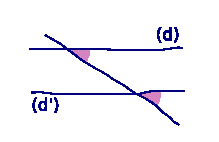
\includegraphics[width=.25\linewidth]{qcm3}
\end{center}
\begin{ChoixQCM}{4}
\item Si les angles roses sont égaux alors $(d)$ et $(d')$ sont parallèles
\item Si $(d)$ et $(d')$ sont parallèles alors les angles roses sont égaux
\item Les angles roses sont correspondants
\item Les angles roses sont alternes-internes
\end{ChoixQCM}
\begin{corrige}
\reponseQCM{a}
\end{corrige}
\end{exercice}



\begin{exercice}
Quelles sont les affirmations vraies ?
\begin{ChoixQCM}{4}
\item $\widehat{OUG}$ et $\widehat{ZKL}$ sont opposés par le sommet
\item Deux angles alternes-internes peuvent être opposés par le sommet
\item Deux angles correspondants peuvent être opposés par le sommet
\item Le supplémentaire d'un angle aigu est obtus
\end{ChoixQCM}
\begin{corrige}
\reponseQCM{a}
\end{corrige}
\end{exercice}




\begin{exercice}
\begin{center}
    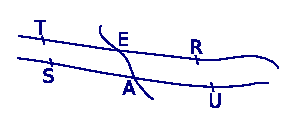
\includegraphics[width=.25\linewidth]{qcm4}
    
    $(TR)$ et $(SU)$ sont parallèles et $\widehat{REA}$=60°.
\end{center}
\begin{ChoixQCM}{4}
\item $\widehat{EAS}=60$°
\item $\widehat{TEA}=120$°
\item $\widehat{EAU}=60$°
\item $\widehat{EAU}=90$°
\end{ChoixQCM}
\begin{corrige}
\reponseQCM{a}
\end{corrige}
\end{exercice}

\end{GroupeQCM}
\end{QCM}